\chapter{Analyse der Informationsquellen in einem industriellen Produktionsnetzwerk}
In diesem Kapitel soll in Folge der Analyse der relevanten Informationsmenge in Unternehmensnetzwerken eine Betrachtung des Zustandes in industriellen Produktionsnetzwerken erfolgen. Als industrielles Produktionsnetzwerk werden dafür in diesem Kapitel die Netzwerkstrukturen in der Produktionsleit- und Feldebene betrachtet.

\label{cha:Analyse der Informationsquellen in einem industriellen Produktionsnetzwerk}
%Ziel der Analyse
Wie bereits im vorherigen Kapitel ist das Ziel der Analyse, die sicherheitsrelevante Infortmationsmenge zu erfassen. Informationen werden als sicherheitsrelevant betrachtet, wenn diese Informationen genutzt werden können, um die Nutzung eines bestimmten Angriffsvektors erkennen zu können. Da automatisierte Anlagen abhängig vom Industriezweig und selbst von Unternehmen zu Unternehmen zweckgebunden unterschiedlich sind, wird ein stark vereinfachtes Modell ausgewählt, welches die Elemente eines Automatisierungsnetzwerkes zeigt. Da das grundlegende Ziel die Ermittlung der Informationsmenge ist, werden Elemente wie etwa die weite Verteilung / Verbreitung von Fertigungssystemen in diesem Kapitel nur am Rande berücksichtigt. 

\begin{figure}[h]
\centering
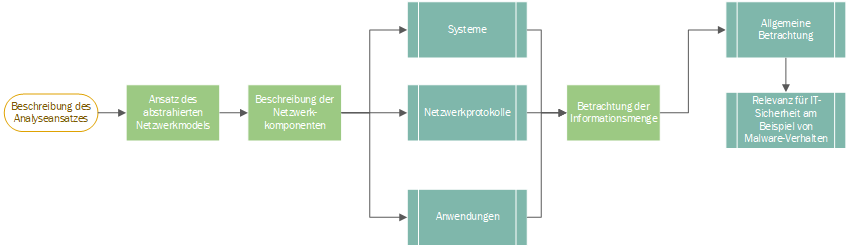
\includegraphics[width=125mm]{Zeichnungen/Analyseansatz.png}
\caption{Analysestruktur (Placeholder)}
\label{fig:Analyseansatz (Placeholder)}
\end{figure}

%Beschreibung der Durchführung
Äquivalent zu der Betrachtung der Unternehmensnetzwerke werden das benutzte Modell und dessen Komponenten beschrieben. Das Ziel der Beschreibung der Komponenten ist eine grobe Klassifizierung der verfügbaren Informationsquellen der Komponenten. Da in industriellen Netzwerken konkurrierende Standards und viele proprietäre Protokolle und Geräte verwendet werden, muss eine Einschränkung stattfinden. Deswegen fällt die Auswahl für die Modellkomponenten auf populäre Elemente des europäischen Raum. Desweiteren wird basierend auf der individuellen Natur der Programmierungen und Parameteranpassungen auf den zu steuernden Prozess der Fokus der Beschreibungen basierend auf der betrachteten Komponente angepasst.

Danach werden die ermittelten Informationsquellen zu den im letzten Kapitel etablierten Informationskategorien zugeordnet. Dies ermöglicht den Vergleich der Informationsmengen.

\section{Beschreibung der Unternehmensarchitektur (Beispiel)}

\todoForm{Industrienetzwerk: Bild zum Model einfügen}
Das verwendete Modell bezweckt die Darstellung des Pfades vom Leitsystem (inklusive eines SCADA Systems) zu den Elemente der Feldebene (SPS und Aktoren/Sensoren). Das Leitsystem wird mit einem Industrie-PC in der Funktion eines Servers für die Datenabfrage aus der Feldebene verbunden. Das SCADA System wird durch das Siemens WinCC System dargestellt. Für die Kommunikation zwischen Server und der Kontrolleinheit des Prozesschrittes (SPS) wird das Industrial Ethernet Protokoll PROFINET eingesetzt. Für die Kommunikation mit den Pheripheriegeräten wird das Feldbussystem PROFIBUS genutzt. Als SPS wird eine Siemens S7 eingesetzt.

\subsection{Systeme}
\subsubsection{SIMATIC S7-1200 (SPS)}
Die SIMATIC S7-1200 wird als Beispiel für eine gebräuchliche SPS herangezogen. Wie im Grundlagenkapitel bereits erläutert, wird die Funktionsweise der SPS durch die Firmware für die unterliegenden Funktionen des Ansprechens der Baugruppen und der Zentralen Einheit (CPU) und das Anwenderprogramm bestimmt. Basierend auf diesem Zustand ist es nicht möglich, eine allgemeine Aussage darüber zu treffen, welche Daten grundsätzlich protokolliert und verfügbar gemacht werden können. Aus diesem Grund widmet sich diese Beschreibung genauer den verfügbaren Befehlen und Optionen der SPS und der SPS-Programmierung, um eine Abschätzung der verfügbaren Datenmenge und Art der Daten vorzunehmen.\\ 

%Quelle: https://www.siemens.com/global/de/home/produkte/automatisierung/systeme/industrie/sps/s7-1200.html
Grundlegend besteht die S7-1200 aus den folgenden Baugruppen:
\begin{itemize}
\item Zentralbaugruppe (CPU): Ausführung des Anwenderprogrammes
\item Signalbaugruppen: Schnittstellen zu den Aktoren und Sensoren
\item Kommunikationsbaugruppen: Erweiterung der SPS um weitere Kommunikationsschnittstellen
\item Technologiebaugruppen: Erweiterung der SPS um spezielle Funktionen (z.B. das Messen von Energiedaten)
\end{itemize}

Basierend auf dieser Auflistung wird für eine gemeinsame Grundmenge im Folgenden auf die Zentralbaugruppe eingegangen \citep{SiemensSPS1}. Für diese Beschreibung wurde als Quelle das Betriebshandbuch \citep{SiemensSPS2} verwendet. \\

%Handbuchquelle: https://support.industry.siemens.com/cs/document/109741593/simatic-s7-s7-1200-automatisierungssystem?dti=0&dl=de&lc=en-WW
Grundlegend nutzt man für die Programmierung einer SPS Programmbausteine. Diese dienen dem Zweck der Steuerung und Ausführung des Anwenderprogrammes. Grundsätzlich wird zwischen den folgenden Bausteinen unterschieden:
\begin{itemize}
\item Organisationsbausteine (OBs): Diese Bausteine legen die Struktur des Programmes fest und fungieren für den Aufruf und die Ausführung bestimmter Unterprogramme und Alarme
\item Funktionsbausteine (FBs) und Funktionen (FCs): Funktionen werden etwa durch die CPU bereitgestellt. Sowohl FBs als auch FCs enthalten ausführbare Programmcodes, der für die Ausführung einer bestimmten Aktion und die Definition von E/A-Parametern im Umgang mit bestimmten Modulen genutzt wird. 
\item Datenbausteine (DBs): Datenbausteine werden für die temporäre Speicherung von Daten (z.B. Rechnungsergebnissen) verwendet. DBs können auf verschiedenen Ebenen eingesetzt werden, wodurch der Zugriff auf die Daten durch andere Funktionsbausteine oder Programme möglich wird.
\end{itemize}

Diese Bausteine werden relevant u.a. im Bezug auf die Interaktion mit den Betriebszuständen der CPU. Die Steuerung der Programmausführung durch die OBs umfasst u.a. die folgenden Bereiche: Strukturierung des Programmzyklus, Strukturierung des Anlaufes, Strukturierung des Aufrufes von Alarmen (Weckalarm, Prozessalarm, Zeitfehler und Diagnosefehler). Dies ist u.a. deshalb relevant, weil Fehlerereignisse in den Diagnosepuffer eingetragen und über eine Schnittstelle abgerufen werden können. \\

Für die CPU sind die folgenden Betriebszustände definiert:  
\begin{itemize}
\item STOP: Programm wird nicht ausgeführt, Laden eines neuen Programmes ist hier möglich
\item STARTUP: Einmalige Ausführung von OBs, die für den Anlauf des Programmes notwendig sind
\item RUN: Ausführung des Programmes in einem sich wiederholenden Zyklus
\end{itemize}

Basierend auf diesen Zuständen kann die Ausführung eines Anwenderprogrammes gesteuert werden. Treten Fehler auf, können diese Ereignisse u.a. in den Diagnosepuffer geschrieben werden. Ein Diagnoseereignis wird durch Datum, Uhrzeit, Kategorie und Beschreibung des Ereignis beschrieben. Ereigniskategorien sind bspw. Systemereignisse, CPU-Fehler und Modulfehler, die durch Diagnosefunktionen ermittelt werden. Zudem wird jede Änderung des Betriebszustandes protokolliert. Der Diagnosepuffer speichert die neuesten fünfzig Ereignisse. \\

Für die Parametrierung und den Zugriff auf Daten ist es essentiell, den Datenspeicher und seine Bereiche zu betrachten. Für den Zugriff auf bestimmte Daten ermöglicht die Programmierumgebung für die Steuerungslogik, \glqq STEP7\grqq , das Binden von Datenadressen an symbolische Namen, äquivalent zu Variablen in höheren Programmiersprachen. Der Speicher wird unterteilt in die folgenden Bereiche:
\begin{itemize}
\item E: und A: - Prozessabbild der Eingänge und Ausgänge
\item M: Merker (Elemente, die für das temporäre Speichern von Zwischenergebnissen genutzt werden)
\item DB: Zugriff auf einen Datenbaustein
\end{itemize}

Bzgl. des Zugriffes auf die Ein- und Ausgänge ist es zudem möglich, direkt auf die physischen Eingänge und Ausgänge zuzugreifen. Das Schreiben von Daten ist jedoch nur für die Ausgänge möglich, da die Eingänge direkt mit den Sensoren und Aktoren verbunden sind und die enthaltenen Zustände dementsprechend nicht überschrieben werden dürfen. \\

\textbf{Informationen und Ereignisse}

Im Folgenden wird basierend auf den verfügbaren Anweisungsmöglichkeiten und Funktionen eine Auflistung der potentiellen Daten vorgenommen. Für diese Arbeit wurden die folgenden Kategorien definiert:
\begin{itemize}
\item Potentielle Systemereignisse basierend auf Änderungen der Systemkonfiguration
\item Fehlerereignisse basierend auf Funktionalitäten
\item Fehlerereignisse basierend auf Kommunikationsaktivitäten
\end{itemize}

Eine Auswahl an potentiell wichtigen Informationen wird in der folgenden Tabelle dargestellt. Die Limitierung durch die maximale Größe des Anwendungsprogrammes und des Speichers wird in diesem Abschnitt noch nicht berücksichtigt. 
\todoForm{SIMATIC S7: Tabelle erstellen und Listen ersetzen}
\begin{itemize}
\item Kommunikation: 
\begin{itemize}
\item PROFINET / PROFIBUS Analysefunktionen 
\begin{itemize}
\item Verbindungsinformationen (MAC-Adresse, IP-Adresse oder Busadresse, Spezifikationen des Gerätes)
\item Auslesen der Diagnoseinformationen mit GET\_ DIAG
\item Abrufen der Betriebszustände von Peripheriegeräten oder Modulen
\item Abrufen von LED-Zuständen
\end{itemize}
\item Fehler bei Zugriffen auf die Peripherie
\end{itemize}

\item System:
\begin{itemize}
\item Änderung der System- oder Lokalzeiten
\item Weck- und Verzögerungsalarme (Auslöser für die Ausführung eines Programmteils)
\item (De-)Aktivierung von Unterprogrammen (durch Fehlerereignisse von Alarm-OBs)
\item Ziehen / Stecken-Ereignisse beim Entfernen / Hinzufügen von Baugruppen
\item Fehler bei Baugruppenträgern 
\item Gemeinsame Fehlercodes für erweiterte Anweisungen bzgl. E/A-Ereignissen und Zugriffe auf DBs
\end{itemize}

\item Funktionalitäten:
\begin{itemize}
\item Diagnosefehler
\item Ereignisse bzgl. des Zugriffsschutz der CPU und bestimmter Bausteine
\end{itemize}
\end{itemize}
\todoForm{SIMATIC S7: Auflistung in Tabellenform überführen}

Basierend auf diesem Ausschnitt wird das Potential der Verfolgung von funktionalen Fehlern im Prozess sowie bei der Prozessausführung dargestellt. Ein besonderes Augenmerk soll desweiteren auf die Möglichkeit der Datenprotokollierung gelegt werden.\\

Die S7-1200 und andere Siemens SPSen unterstützen die Erstellung von Protokolldateien im CSV-Datenformat. Für die Einträge von Daten in diese Protokolldateien werden verschiedene Funktionen für die Erstellung, Schreiben und Schließung dieser Dateien bereitgestellt. Jede Protokolldatei kann maximal 256 Einträge speichern. Über interne Ereignisse lässt sich der Zustand und die Erstellung und Schließung der Dateien kontrollieren. Dabei können mehrere Protokolldateien, maximal jedoch acht verschiedene Dateien, gleichzeitig geöffnet sein. Die Gesamtmenge an Protokolldateien wird durch die Größe des Ladespeichers bzw. einer hinzugefügten Speicherkarte definiert. Die Gesamtmenge darf maximal 25\% des Speichers einnehmen (basierend auf der Größe des Ladespeichers 250-500 KByte / Speicherkarte bis zu 6 MByte). Der Zugriff auf die Protokolldateien kann entweder über die Aktivierung des Webservers oder den direkten Zugriff auf Protokolldateien über einen Webbrowser (\glqq http://<IP-Adresse>/DataLog.html?FileName=<Name der Protokolldatei>\grqq ) erfolgen, sofern eine geeignete Verbindung (z.B. über PROFINET) vorhanden ist. 
Protokolldateien werden im Ladespeicher oder auf einer Speicherkarte abgelegt, dürfen jedoch maximal 25\% des jeweiligen Speichers belegen.

%Quelle für Loggingmethoden: https://cache.industry.siemens.com/dl/files/939/109746939/att_936594/v4/109746939_WinCC_TIA_Portal_Archivierung_Komp_DOC_en.pdf


\subsection{Kommunikationsmedien}
\subsubsection{PROFIBUS}
%Quelle:http://www.feldbusse.de/Profibus/profibus.shtml
PROFIBUS ist ein serielles Feldbussystem, welches u.a. in der Fertigungs-, Prozess- und Gebäudeautomatisierung verwendet wird. Es ermöglicht die zeitkritische, deterministische Kommunikation von Steuer- und Peripheriegeräten (Aktoren und Sensoren) sowie HMIs und anderen Elementen. Das Kommunikationsprinzip basiert auf dem Multi-Master-Prinzip. Dies soll den gemeinsamen Betrieb mehrerer Systeme für den Zweck der Automatisierung, des Engineerings oder der Visualisierung der Anlage, mit den verteilten Pheripheriegeräten der Anlage ermöglichen. Zu diesem Zweck werden die Kommunikationsteilnehmer in zwei Gerätearten unterteilt: Master- und Slave-Geräte. Master-Geräte bestimmen die Kommunikation und senden auf dem Feldbus, wenn sie im Besitz des Tokens sind, welches das Zugriffsrechte auf den Datenbus darstellt. Slave-Geräte hingegen können lediglich empfangene Nachrichten bestätigen oder auf Anfrage des Master-Gerätes Daten senden\citep{Profibus1}.\\

Für die Datenübertragung werden drei Versionen von PROFIBUS DP verwendet. DP-V0 dient der zyklischen, DP-V1 und DP-V2 der azyklische Kommunikation.\\

\textbf{Fieldbus Data Link: Datenübertragung in PROFIBUS}

%http://www.feldbusse.de/Profibus/Buszugriffsprotokoll.shtml
Für die Zuweisung der Buszugriffsrechte, Verwaltung und Durchführung der Datenübertragung wird das \textit{Fieldbus Data Link} (FDL) Protokoll verwendet. Dieses verbindungslose, Layer-2-Protokoll bestimmt, zu welchem Zeitpunkt ein bestimmter, aktiver Kommunikationsteilnehmer (Master) das Recht erhält, Daten zu senden. Die dadurch etablierte Buszugriffskontrolle (MAC, Medium Access Control) führt die folgenden Aufgaben aus:
\begin{itemize}
\item Etablierung des Token-Rings während des Hochfahrens des Systems
\item Hinzufügen/Entfernen von Teilnehmern
\item Kontrolle der Weitergabe des Tokens
\end{itemize}
\citep{Profibus2}

Der Token-Ring wird durch aufsteigende Busadressen der Master-Geräte realisiert. Die Tokeninformationen werden durch ein spezielles Telegram weitergegeben. Abhängig von der Definition und Größe des Systems muss das Token in einer maximalen Token-Umlaufzeit einmal an jeden aktiven Kommunikationsteilnehmer weitergesendet werden. Dieses Verfahren ermöglicht die Erstellung von Master-Slave-, Master-Master- und Misch-Kommunikationsformen. Die Adressierung wird durch einen Byte-Wert zwischen 0 und 127 kodiert. Dabei werden bestimmte Bereiche für etwa Programmiergeräte, Slaves und Master bestimmt \citep{Profibus2}.

Desweiteren wird durch eine Unterscheidung der verschickten Telegramme (Nachrichten) eine logische Datensicherung etabliert. Diese wird durch bestimmte Start- und Endzeichen sowie Paritätsbits und Kontrollbytes hergestellt \citep{Profibus2}.

%Dienste der Datenübertragung: https://www.profibus.felser.ch/datenubertragung_1.html
Für die Übertragung von Daten werden verschiedene Dienste verwendet. Abhängig von der benutzen Version des PROFIBUS DP (V0, V1, V2) Protokolls stehen unterschiedliche Dienste zur Verfügung, dazu zählen u.a.:
\glqq 
\begin{itemize}
\item SDN (Send Data with No acknowledge, alle Versionen)
\item SRD (Send and Request Data, alle Versionen)
\item CS (Clock Synchronisation, DP-V1 und DP-V2)
\item MSRD (Send and Request Data with Multicast Reply, DP-V2)
\end{itemize}
\grqq
\citep{Profibus7} 


%Quelle: https://www.profibus.felser.ch/telegrammformate.html
Für die PROFIBUS-Protokolle der Anwendungsebene (DP-Varianten) werden verschiedene Telegramformate bereitgestellt:
\begin{itemize}
\item Keine Daten (SD1)
\item Daten variabler Länge (SD2)
\item Daten fester Länge (SD3)
\item Token (SD4)
\item Kurzquittung (SC)
\end{itemize}
\citep{Profibus8}

%Telegramme: https://www.profibus.felser.ch/telegrammformate.html
Das Format der Nachricht ist abhängig von dem verwendeten Telegramtyp. Die grundlegenden Header sind:
\begin{itemize}
\item Telegrammformat
\item Empfängeradresse (außer SC)
\item Senderadresse (außer SC)
\item Function Code (Telegramtyp, der die Funktion festlegt)
\end{itemize}
\citep{Profibus8}

%Quelle:  https://www.profibus.felser.ch/fdl_parameter.html
Zusätzlich zu der Diensten der Datenübertragung existieren die Fieldbus Management (FMA) Dienste für die Verwaltung der Schichten 1 (Übertragungstechnik) und 2 (FDL). Diese Dienste können unterteilt werden in lokale Dienste (bzgl. der Station) und stationsübergreifende Dienste. Zu den lokalen Diensten zählen \glqq Reset\grqq , \glqq Set Value\grqq , \glqq Read Value\grqq , \glqq (R)SAP (De-)Activate\grqq  und \glqq Event\grqq . Event ist ein Dienst, der Anwender über Ereignisse oder Fehler in den Schichten 1 und 2 informieren kann. Zu diesen Events zählen:
\begin{itemize}
\item Duplicate adress (Master)
\item Faulty transceiver (Master)
\item Time\_put (Master / Slave)
\item Not\_syn (Master / Slave)
\item Out\_of\_ring (Master
\item GAP\_event (Master)
\end{itemize}

Zu den stationsübergreifenden Diensten zählen \glqq Ident (Versionsdaten von Hardware und Software)\grqq , \glqq LSAP Status (Informationen zu einem SAP)\grqq  und \glqq Live-List (Liste aller erreichbaren Teilnehmer)\grqq \citep{Profibus12}.\\

\textbf{PROFIBUS DP-V0: Zyklische Kommunikation}

%http://www.feldbusse.de/Profibus/Profibus-DP.shtml
PROFIBUS DP dient als Protokoll für den zyklischen Datenaustausch zwischen einer Kontrolleinheit (SPS) und Peripheriegeräten. Bei der Verwendung von DP wird zwischen drei Gerätetypen unterschieden:
\begin{itemize}
\item DP-Master 1 (DPM1): Dieser Kommunikationsteilnehmer regelt den zyklischen Datenaustausch (typischerweise SPS oder PC)
\item DP-Master 2 (DPM2): Ein zusätzliches Gerät, etwa für Bedienungs- oder Engineering-Zwecke, die Kommunikation erfolgt azyklisch
\item Slave: Pheripheriegeräte (Aktoren/Sensoren)
\end{itemize}

PROFIBUS DP unterstützt Mono- und Multi-Mastersysteme. Ein Multi-Mastersystem besteht aus verschiedenen Subsystemen (Mono-Master, d.h. DPM1 mit mehreren Slaves) und weiteren DPM2-Geräten. Die Kommunikation wird mit Hilfe des FDL Protokolls geregelt \citep{Profibus5}.


Das Verhalten eines (Sub-)Systems hängt von dem Betriebszustand des DPM1 ab. Es wird zwischen den folgenden Betriebszuständen unterschieden:
\begin{itemize}
\item Stop: Kein Datenverkehr zwischen DPM1 und Slaves
\item Clear: DPM1 liest Eingangsinformationen der Slaves und schaltet die Ausgänge in einen sicheren Zustand
\item Operate: Zyklische Kommunikation zwischen DPM1 und Slaves (Datentransferphase)
\end{itemize}

Bei der zyklischen Kommunikation im \glqq Operate\grqq -Zustand sendet (schreibt) der Master per Aufruf-Telegramm Ausgangsdaten an den jeweiligen Slave und empfängt (liest) die Eingangsdaten des Slaves. Dieser Vorgang wiederholt sich in dieser Reihenfolge konsequent. Wird ein neuer Slave in das System eingefügt, werden drei Phasen durchlaufen: Parametriesierungs-, Konfigurations- und Datentransferphase. Die ersten Phasen dienen einem Ist-Soll-Abgleich zwischen DPM1 und Slave, bei dem der DPM1 Gerätetyp, Format- und Längeninformationen sowie die Anzahl der Ein- und Ausgänge prüft. Nach erfolgreicher Prüfung geht die Kommunikation in die Datentransferphase über \citep{Profibus5}. 

Neben dem Datenaustausch zwischen einem DPM1 und einem einzelnen Slave besteht auch die Möglichkeit eines Multicasts, bei dem Steuerungsbefehle an einen, eine Gruppe oder alle Slaves des von dem DPM1 verwalteten System gesendet werden können. Diese Funktionalität ermöglicht die Betriebsarten Sync und Freeze. 
Bei der Sync-Betriebsart werden zunächst die Ausgangszustände der Slaves eingefroren, d.h. sie können nicht mehr verändert werden. Darauf werden Ausgangsdaten vom DPM1 auf dem Slave gespeichert, die Zustände jedoch nicht verändert. Durch einen erneuten Sync-Befehl werden die Zustände überschrieben. Ein Unsync-Befehl beendet den Sync-Betrieb.
Bei der Freeze-Betriebsart werden die Eingangszustände der Slaves eingefroren. Die Eingangszustände werden aktualisiert, sobald ein weiterer Freeze-Befehl gesendet wurde. Analog zu Sync wird der Freeze-Betrieb durch den Unfreeze-Befehl beendet \citep{Profibus5}.


Für den Schutz gegen Fehlparametrierung, d.h. falscher Setzung der Operationsparameter, und Ausfall des Übertragungsmediums, werden für DP-Master als auch DP-Slaves \glqq Data\_ Control\_ Timer\grqq{}  ausgelöst, sobald innerhalb eines festgelegten Zeitintervalls keine ordnungsgemäße Kommunikation stattgefunden hat. Im Fall des DP-Masters kann zu diesem Zweck der Parameter \glqq Auto-Clear\grqq{}  aktiviert (True) sein. In diesem Falle werden die Ausgänge aller Slaves in einen sicheren Zustand geschaltet und daraufhin der Clear-Betriebszustand eingenommen \citep{Profibus5}. \\

%Betriebszustände Slaves und Einbindung: https://www.profibus.felser.ch/ms0_zyklischer_datenaustausch.html
Neben den Betriebszuständen der PROFIBUS-Master-Geräte nehmen auch die PROFIBUS-Slave-Geräte verschiedene Zustände an: Eingeschaltet, WPRM (Warten auf Parameter), WCFG (Warten auf Konfiguration) und DXCHG (Datenaustausch)\citep{Profibus9}.

%Slave Init
Damit Daten mit einem PROFIBUS-Slave-Gerät ausgetauscht werden können, muss das Gerät in den DXCHG-Zustand wechseln. Um diesen Zustand zu erreichen, wird eine Initialisierungsphase durchgeführt. Zunächst wird die Existenz des Slaves über eine Diagnoseanfrage bestimmt. Daraufhin werden Parameter von dem zuständigen PROFIBUS-Master übertragen und die Konfiguration und Parameter geprüft. Während dieses Prozesses werden die genannten Zustände durchlaufen, bis der Datenaustausch möglich ist\citep{Profibus9}.\\

%Codierung der Diagnose
Für die Analyse von Fehlern stehen Diagnose SAPs (Service Access Points) zur Verfügung. Mit Hilfe dieser Dienste lassen sich Informationen zu Fehlern codiert abfragen. Die Diagnosetelegramme enthalten u.a. drei Statusfelder (je 8 Bit), welche Kommunikationsfehler (Status1), Gerätefehler (Status2) und den Überlauf des Diagnosepuffers (Status3) kodieren\citep{Profibus11}.\\

\textbf{PROFIBUS DP-V1: Azyklische Kommunikation}

%Quelle: http://www.feldbusse.de/Profibus/DPV1.shtml
PROFIBUS DP kann durch PROFIBUS DPV1 erweitert werden. DPV1 dient der azyklischen Kommunikation und ermöglicht die Kommunikation von DPM2-Geräten und Slaves. Die azyklische Kommunikation dient der Übertragung von Bedarfsdaten. Bedarfsdaten sind Parameter (z.B. Grenzwerte) oder Optionen (z.B. Fehlerlisten), die von den Slaves abgerufen werden können. Zu diesem Zweck erweitert DPV1 DP um die folgenden Dienste: \glqq Read\grqq und \glqq Write\grqq \citep{Profibus6}.


Die azyklische Kommunikation wird parallel zur zyklischen Kommunikation durchgeführt. Der Ablauf kann am Beispiel Read demonstriert werden:
\begin{itemize}
\item (Für DPM2: Aufbau einer C2-Verbindung)
\item DP-Master sendet den Aufruf an den DP-Slave
\item Der DP-Slave bestätigt den Erhalt der Anfrage und beginnt die interne Bereitstellung der Daten (Quittierung)
\item DP-Master führt zyklische Prozesskommunikation durch
\item Wiederholend:
\begin{itemize}
\item DP-Master sendet Poll-Request
\begin{itemize}
\item Daten stehen noch nicht bereit? DP-Slave quittiert Poll-Request
\item Daten stehen bereit: DP-Slave sendet Daten an Stelle der Quittierung
\end{itemize}
\end{itemize}
\end{itemize}

Die aufgerufenen Betriebsdaten werden über das Modul (\glqq Slot\grqq ) und den jeweiligen Parameter (\glqq Index\grqq ) definiert. Soll nur ein Teilwert des Parameters gelesen werden, kann über die Länge (\glqq Length\grqq ) dies definiert werden. Die Indexnummern und Datentypen werden in PROFIBUS Profilen festgelegt\citep{Profibus6}.

%Quelle: https://www.profibus.felser.ch/ms1_verbindung.html
Für den azyklischen Datenaustausch müssen zunächst bestimmte Parameter gesetzt und als Konfiguration bestätigt werden. Die Unterstützungsmöglichkeit der azyklischen Kommunikation wird in der GSD-Datei des Gerätes definiert. 

Die Read- und Write-Dienste von PROFIBUS DP-V1 greifen über einen Index auf die Daten zu. Das zugehörige Telegramm enthält den Telegrammformat (\glqq Kurzquittung\grqq -Format), die Slot-Nummer des Moduls, die Indexnummer des Parameters sowie die Länge der Nachricht. Bei einer Antwort werden die Daten angehängt \citep{Profibus11}.


Da die Leistungsmerkmale der Geräte, d.h. Busparameter und Funktionalitäten (z.B. Anzahl der E/A-Signale und Diagnosemeldungen), abhängig von Gerätetyp und Hersteller unterschiedlich sind, werden GSD-Dateien für die Definition dieser Elemente verwendet. Eine GSD-Datei stellt dabei eine Art elektronische Gerätedatenblatt da und kann während der Konfiguration, z.B. durch ein Projektierungswerkzeug, eingelesen werden. Die GSD-Dateien sind in drei Abschnitte eingeteilt:
\begin{enumerate}
\item Allgemeine Festlegungen
\item Master-bezogene Festlegungen
\item Slave-bezogene Festlegungen
\end{enumerate}

Zudem muss in der GSD-Datei eine Identnummer vermerkt sein. Diese Identnummer muss bei der PROFIBUS-Nutzerorganisation beantragt werden und dient der schnellen Identifzierung eines angeschlossenen Gerätetyps durch einen DP-Master \citep{Profibus6}.\\

%Quelle: https://www.profibus.felser.ch/alarmbehandlung.html
Alarm- und Statusmeldungen von PROFIBUS DP-V1 werden im Vergleich zu V0 umfassender beschrieben. Dazu werden die Alarmmeldungen in verschiedene Typen unterteilt, die Sequenz der Telegramme jeweils quittiert und die Daten in komplexeren Strukturen verpackt. Die GSD Datei legt u.a. fest, welche Alarmtypen von dem Gerät unterstützt werden. Für die Übertragung werden die Alarme in Diagnose-Nachrichten verschickt. Diese bestehen aus dem Typ-Header, dem Alarmtyp, Speicherindex, eine 8bit-Spezifizierung über den Zustand des Alarms sowie Diagnosedaten.\\

In der Erweiterung PROFIBUS DP-V2 wird die Uhrensynchronisierung durch den DPM1 und isochrone Kommunikation hinzugefügt. Zum Zweck der Uhrensychronisation wurde der Gerätetyp DP-Master 3 (Uhrenmaster) eingefügt.

%Details aus dem Handbuch: https://www.profibus.felser.ch/fdl_parameter.html
% Für Daten: https://www.profibus.felser.ch/gsd_dateien.html

\subsubsection{PROFINET}
%Quelle: 20180322(Profinet Descriptions)\PROFINET_Systembeschreibung_DT_2014_web.pdf
Profinet ist ein offener Industrial-Ethernet-Standard für die Integration  von IT-Systemen in den Automatisierungsprozess auf Basis von TCP/IP. Für die nachfolgende Beschreibung wird auf die Systembeschreibung der PROFIBUS Nutzerorganisation (PNO)\citep{PROFINET1} zurückgegriffen. \\


Wie bei PROFIBUS werden Kommunikationsteilnehmer in einem Profinet-IO-System in verschiedene Gerätekategorien eingeteilt: IO-Controller (typischerweise eine SPS), IO-Device (Gerät der Feldebene) und IO-Supervisor (Programmiergerät, PC, HMI oder anderes zusätzliches Werkzeug (etwa für Engineering-Zwecke)). Der IO-Supervisor entspricht dem PROFIBUS DP-Master 2. 

Zusätzlich werden wie bei PROFIBUS Geräte- bzw. Anwendungsprofile in Form von GSDML-Dateien verwendet. Diese werden durch den Hersteller erstellt und beschreiben Eigenschaften, Leistungsmerkmale und Verhaltensweise der Geräte. Dabei wird zwischen allgemeinen Anwendungsprofilen mit verschiedenen Einsatzmöglichkeiten und spezifischen Anwendungsprofilen unterschieden. 

Geräte der Feldebene werden durch ihr Gerätemodell beschrieben, welches die technischen und funktionellen Möglichkeiten darlegt. Das Gerätemodell wird definiert durch den Zugriffspunkt (Device Access Point (DAP)) und die für eine bestimmte Gerätefamilie definierten Module (Baugruppen über die die Kommunikation der Prozessdaten abläuft). Der DAP dient als Schnittstelle für die Ethernet-Kommunikation und Verarbeitungsprogramme. Die Module erlauben die Adressierung der E/A-Daten über die Parameter Slot (Steckplatz/Baugruppe), Subslot (Prozess-Schnittstelle, definiert durch den Hersteller), den Index (gibt den Parameter an) sowie den Application Profile Identifier. Diese Daten werden azyklisch per Read/Write ausgelesen.
Der Ausbaugrad eines Anwendungsprofils wird kategorisiert als \glqq kompakt\grqq{}  (nicht-veränderbar) oder \glqq modular\grqq . Die GSDML-Datei wird auf einer XML-Basis erstellt.\\


Die Kommunikationswege innerhalb eines PROFINET-Systems werden auf Basis dieser GSDML-Dateien erstellt während der Projektierung. Der Datenaustausch zwischen Kommunikationsteilnehmern wird innerhalb einer Application Relation (AR) durchgeführt, die verschiedene Communication Relations (CRs) spezifiziert:
\begin{itemize}
\item Recorded Data CR: Standardkanal für Konfigurationsdaten
\item IO Data CR: Kanal für die zyklische Übertragung von Echtzeitdaten
\item Alarm CR: Kanal für Alarme und Fehlermeldungen
\end{itemize}

Sollen mehrere IO-Controller auf die gleichen Daten eines IO-Device zugreifen, muss dieses während der Projektierung angegeben werden. Jeder IO-Controller kann genau eine AR zu einem bestimmten IO-Device aufbauen. Jedes Feldgerät erhält zudem einen symbolischen Namen als Identifier, welcher als Schlüssel für die Zuordnung von MAC- und IP-Adresse verwendet wird. Die Zuordnung dieses Namens kann über das \glqq Discovery and basic Configuration (DCP)\grqq{} Protokoll, alternativ aber auch über die Topologie und Nachbarschaft zu einem bestimmten IO-Controller, durchgeführt werden. Die Zuweisung der IP-Adresse wird per DHCP oder einen herstellerspezfischen Mechanismus durchgeführt. Die verwendbaren Möglichkeiten sind innerhalb der GSDML-Datei definiert.

Für die Adressierung innerhalb des PROFINET-Systems werden eindeutige 48-Bit-MAC-Adressen verwendet. Die MAC-Adresse wird zusammengesetzt aus der Firmenkennung und einer Organization Unit ID (OUI), welche gegen eine Gebühr von IEEE-Departments vergeben werden.\\


Der Funktionsumfang von Profinet ist flexibel anpassbar abhängig von der notwendigen Funktionalität. Für eine Differenzierung der Funktionalitäten teilt man Profinet in die folgenden Konformitätsklassen ein:
\begin{itemize}
\item CC-A: Grundfunktionen
\item CC-B: CC-A wird um Netzwerkdiagnose und Topologieinformationen erweitert
\item CC-B(PA (Process Automization)): CC-B wird um Systemredundanzen erweitert
\item CC-C: Basisfunktionen für Geräte und hardwareunterstützte Bandbreitenreserver für isochrone Echtzeitkommunikation (Basis für taktsynchrone Anwendungen)
\end{itemize}


\textbf{Grundfunktionen}


Die Grundfunktionen umfassen den zyklischen Austausch von E/A-Daten mit Echtzeiteigenschaften sowie azyklische Kommunikation (Read/Write) von bedarfsorientierten Daten (Parameter, Diagnose) sowie Identifizierungs- und Verwaltungsfunktionen (Identification and Maintenance (I\&M)) und eine Alarmfunktionalität für die Signalisierung von Geräte- und Kommunikationsfehlern. Für die Identifzierung eines Gerätes werden die folgenden Elemente verwendet: MAC-Adresse, Hardware-Version, Software-Version, Produkttyp und Hersteller-ID. Neben diesen Informationen lassen sich weiter Informationen auf Geräte- oder Modullevel abrufen\citep{PROFINET2}.


Der zyklische Datenaustausch wird über eine IO Daten CR auf Layer 2 des OSI-Modells in einem Zeitfenster zwischen 250 $\mu $s und 512ms durchgeführt. Die gesendeten Daten werden durch den Empfänger nicht bestätigt. Die Telegramme enthalten neben den Prozessdaten weitere Informationenen für die Bestätigung der Gültigkeit der Daten, Redundanz- und Diagnosedaten sowie Informationen über den Taktzyklus des Providers. Wie auch bei PROFIBUS werden die Zeitintervalle zwischen den Kommunikation überwacht und Mechanismen ausgelöst, falls der Zeitabstand überschritten werden sollte. 

Der azyklische Datenaustausch wird über die Record Data CR auf Basis von TCP/IP durchgeführt. Die Read/Write-Rahmen werden verwendet, um Diagnose- und Identifzierungsinformationen über das Netzwerk und die Kommunikationsteilnehmer abzurufen. Die Diagnosedaten enthalten u.a. mehrstufige Alarmereignisse. Das Zustandsmodell unterscheidet zwischen den Kategorien \glqq gut\grqq , \glqq Wartungsbedarf (etwa bei einem Ausfall der Medienredundanz-Funktionalität)\grqq , \glqq Wartungsanforderung\grqq{} und \glqq fehlerhaft\grqq . Zudem wird zwischen Diagnose- und Prozessalarmen unterschieden. Diagnosealarme umfassen Fehler oder Ereignisse, wie etwa das Abziehen oder Aufstecken einer Baugruppe, innerhalb des IO-Devices und im Bezug auf zusammenhängende Komponenten. Prozesslarame werden durch den Anwender definiert und signalisieren etwa die Überschreitung eines Grenzwertes. \\


\textbf{Netzwerkdiagnose und -verwaltung (CC-B)}


Die Konformitätsklasse (CC) B erweitert PROFINET um weitere Diagnoseinformationen und Topologieinformationen. Diese Informationen werden durch die Erweiterung des Link Layer Discovery Protocols (LLDP-MIB EXT) und innerhalb einer Management Information Base (MIB) gesichert. Die Informationen sind abrufbar über die Verwendung des Netzwerkprotokolls SNMP oder die Verwendung azyklischer Profinet-Dienste. 

Die Erweiterung um Informationen der Topologie des Netzwerkes wird durch die Nachbarschaftserkennung ermöglicht. Durch diese Erweiterung tauschen PROFINET-Feldgeräte über LLDP vorhandene Adressierungs-Informationen aus, wodurch der phyikalische Aufbau auf Basis der Port-Nachbarn erschlossen wird. Diese Funktionalität ermöglicht einen Soll-Ist-Vergleich der Topologie sowie die Prüfung des korrekten Anschlusses für den Falls des Austausches eines Gerätes mithilfe eines Software-Werkzeuges. 

Für die Verwendung dieser Erweiterung müssen die Switche als IO-Device eingesetzt werden können, um die Übertragung der Alarme über die Alarm CR zu ermöglichen. \\


\textbf{Synchrone Echtzeit (CC-C)}

Um PROFINET für zeitkritische, deterministische Kommunikation nutzen zu können, müssen weitere Funktionalitäten hinzugefügt werden. Dies umfasst eine netzwerkweite Synchronisierungsfunktion und zeitliche Übertragungsschwankungen (\glqq Jitter\grqq ) von weniger als 1 ms. Zu diesem Zweck wird eine definierte Bandbreite für das Übertragen dieser Daten reserviert, während die restliche Bandbreite für den restlichen Datenverkehr genutzt wird. Die synchrone Kommunikation erfordert, dass alle Kommunikationsteilnehmer den gleichen Takt verwenden. Dies wird über einen Clock-Master für alle lokalen Taktgeneratoren innerhalb des Taktystems (IRT Domäne) umgesetzt. Zwischen den beteiligten Geräten dürfen keine asynchronen Geräte verwendet werden. Um die Schnelligkeit der Übertragung zu verbessern, verwendet man verschiedene, zusätzliche Mechanismen (Fragmentierung in kleinere TCP/IP-Pakete sowie Dynamic Frame Packing (DFP)). 

%Was fehlt: Ablauf der Profinet-Kommunikation, Aufbau eines Profinet-Datenpaketes

\section{Applikationen}
\subsection{WinCC (SCADA / HMI)}
%Quellen: 
%Getting-Started Dokument, 
%https://mall.industry.siemens.com/mall/de/WW/Catalog/Products/10042373?tree=CatalogTree
Als Beispiel für das SCADA-System wird in diesem Modell das System \glqq WinCC\grqq{} von Siemens verwendet. WinCC ist ein pc-basiertes System, das sowohl als eigenständiges SCADA-System als auch als HMI für Prozessleitsysteme eingesetzt werden kann. WinCC wird auf einer modernen Version des Betriebssystem Windows ausgeführt (z.B. Windows 7, 8.1 oder 10 sowie Windows Server 2008 oder 2016). Mit Hilfe dieses Systems ist es möglich, die Durchführung und Überwachung eines Fertigungsprozesses durchzuführen\citep{WinCC2}. Dies beinhaltet im Kern die folgenden Funktionalitäten\citep{WinCC1}:
\begin{itemize}
\item Meldung und Bestätigung von Ereignissen innerhalb des Fertigungsprozesses
\item Archivierung von Meldungen und Messwerten
\item Protokollierung von gesendeten Prozessdaten und Konfigurationsdaten
\item Grafische Darstellung des überwachten Netzwerkes
\end{itemize}


Hinzu kommen Elemente wie etwa eine Benutzerverwaltung für den geregelten Zugriff auf das System.

Im Bezug auf die für diese Arbeit relevante Informationsmenge ist die Protokollierung und Überwachung des Systems und des Netzwerkes interessant. Da das Betriebssystem bereits im vorherigen Kapitel ausführlich beschrieben wurde, wird im Folgenden das System \glqq WinCC\grqq{} selbst betrachtet und die potentiellen Quellen für Informationen bzgl. des Systems selbst. Das SCADA-System empfängt und sendet Prozessdaten und definierte Bedarfsdaten (Parameterdaten der Steuerungen). Deshalb werden außerdem die Schnittstellen für das Senden und Empfangen der Daten betrachtet.

In WinCC lassen sich die Daten in die folgenden Gruppen unterteilen: Tags, Nachrichten und Alarm Logging. 


In WinCC werden \glqq Tags\grqq{} als Elemente benutzt, um Daten eines Projektes zu lesen, zu schreiben oder weiterzuleiten. Jeder Tag wird mit einer Datenadresse, einem symbolischen Namen und einem Datentyp sowie weiteren Eigenschaften definiert.

Es wird zwischen Prozesstag und internen Tags unterschieden. Ein Prozesstag ist mit einem bestimmten Parameter eines Automatisierungssystems (z.B. einer SPS) verknüpft und definiert u.a. den Kommunikationstreiber, der die Details der Kommunikation definiert. Diese Verbindung wird genutzt, um Daten auszulesen und zu schreiben. Ein interner Tag wird genutzt, um innerhalb des Projektes Daten zu verwalten und dient zudem als Schnittstelle zur Archivierungsfunktion. Interne Tags, die für die Verwaltung des Projektes notwendig sind, werden Systemtags genannt\citep{WinCC3}. \\

Für die Feststellung, Darstellung und Archivierung von Fehlern wird das Nachrichtensystem (Message System) verwendet, um erkannte Fehler visuell darzustellen und an das Archivierungssystem weiterzuleiten. Die Nachrichten werden in drei Teile unterteilt: Systemblocks (Datum, Zeit, Dauer,...), User Text Blocks (vor-definierte Beschreibungen) und Process Value Blocks (Tag-Werte). Zudem wird jede Nachricht einem Typ zugeteilt: Operationsnachrichten (Status eines Prozesses), Fehlernachrichten (Fehler in einem Prozess) und Systemnachrichten (Fehler von anderen Anwendungen).
Dokumentierte Ereignisse schließen binäre Ereignisse (Statusänderungen von Tags) sowie \glqq Monitoring Events\grqq{} (Archivfehler, Serverfehler, Fehler in der Prozesskommunikation) ein. Für die Archivierung werden Prozessdaten und Nachrichten für den Status der Operation und von Fehlern in einem Microsoft SQL Server gesichert \citep{WinCC3}.

\todoQuestion{Beschreibung der WinCC Daten ggf. weiter ausführen? (prüfen)} 


\section{Analyse der Informationsmenge}
Nach der Beschreibung der Elemente des Modells wird numehr eine Zusammenfassung der gesammelten Informationsquellen erfolgen. Um diese Sammlung der Informationsquellen vergleichbar zu machen, werden sie den Kategorien des Unternehmensnetzwerkes zugeordnet (vgl. Analyse des Unternehmensnetzwerkes). Damit schafft man eine Vergleichsbasis der Informationsmengen.

\subsection{Betrachtung der Datenmenge}
Die Betrachtung der ausgewählten Elemente zeigt eine Datenmenge, die sich hauptsächlich auf die Dokumentierung und Analyse des Fertigungsprozesses bezieht. Die verfügbaren Diagnosefunktionalitäten durch die genutzten Kommunikationssysteme PROFINET und PROFIBUS sowie die Diagnose und Alarmierungsfunktionalitäten der SPS und die Abfrage entsprechender Parameter-Tags sowie die Möglichkeit der Speicherung und statistischen Analyse der Prozessdaten ermöglichen eine präzise Kontrolle des Prozesses. Basierend auf den verfügbaren Bausteinen und Parametern der SPS und der Protokollierung von Parametern besteht die Möglichkeit genau festzulegen, welche Daten wichtig für die Überwachung eines Prozessschrittes sind. IT-Sicherheitsfunktionen werden in Form von Zugriffskontrollen der Benutzerverwaltung und Passwortschutz auf wichtige Komponenten umgesetzt. Desweiteren bieten sich die bereits diskutieren Möglichkeiten für die Systemüberwachung des SCADA-Servers durch das Windows-Betriebssystem an. Die Protokollierung von SCADA-Ereignissen ist eingeschränkt möglich, eine genauere Betrachtung ist u.U. im späteren Verlauf zu untersuchen.

\subsection{Kategorisierung der Informationsmenge}
Bei der folgenden Kategorisierung der Informationsmenge sollen die beschriebenen Informationsquellen und Informationen in die im vorherigen Kapitel beschriebenen Kategorien übertragen werden. Daher wird auch hier unterschiedenen zwischen Netzwerkprotokollen und Systemen. Die gewählten Zuweisungen und die zugehörigen Begründungen werden nun dargelegt.

\subsection{Systeme}
%SCADA-Kategorisierung
\textbf{WinCC (SCADA-System)}
Zunächst soll hier die SCADA-Anwendung betrachtet werden. Diese wird auf der Basis von Windows ausgeführt. Aus diesem Grund gelten für das zugrundeliegende Betriebssystem die bereits im vorherigen Kapitel beschriebenen Zuweisungen. Die Anwendung selbst ermöglicht die Abfrage von Prozessdaten aus dem Netzwerk sowie die Protokollierung von empfangenen und gesendeten Prozessdaten und Konfigurationsdaten. Diese Informationen im Bezug auf das ausführende System werden der Anwendungskategorie zugeordnet. Die Entscheidung über die Zuordnung zu der Anwendungskategorie basiert in diesem Falle darauf, dass diese Informationen von WinCC verwendet werden und keine Informationen über das System selbst enthalten. Die internen Tags werden ebenfalls der Anwendungskategorie zugeordnet.\\
\todoQuestion{Industrieanalyse Kategorisierung: Sind gesendete und empfangene Konfigurationsdaten wirklich als Anwendungsdaten zu betrachten? Warum? Warum nicht?} 

%SPS-Kategorisierung
\textbf{Siemens S7-1200 (Speicherprogrammierbare Steuerung)}

Die Informationen der beschriebenen SPS lassen sich in mehrere Kategorien einordnen. So lassen sich potentiell verschiedene Informationen über das System selbst ermitteln, inklusive des Betriebszustandes, Systemzeit und Fehlerereignissen aus dem Diagnosepuffer, etwa Nachrichten bzgl. des Hinzufügens oder Entfernens einer Baugruppe, CPU-Fehler und Modulfehler. Daher werden diese Informationen der Systemkategorie zugeordnet. \\

Alarmereignissen der Zugriffschutzfunktionen können mit der Kategorie \textit{Benutzer} verbunden werden. Diese Informationen bezeichnen ein Ereignis bzgl. des Zugriffs auf abgelegte Daten des Systems. Während diese Informationen auch der Systemkategorie zugeordnet werden könnten, wird hier der Zugriff auf ein \glqq Objekt\grqq{} betrachtet, welches Ähnlichkeiten etwa zu Ereignissen des Sicherheitsprotokolls von Windows aus der Kategorie \glqq Object Access\grqq{} aufweist. 

Weckalarmdaten aus den Organisationsbausteinen werden der Prozesskategorie zugeordnet. Diese geben Informationen über den Start eines Programmes, welches äquivalent zu dem Start eines Prozesses bzw. einer Anwendung in einem Betriebssystem betrachtet wird.\\

Die Prozessdaten aus den Prozessabbildern, die u.a. vom SCADA-System abgefragt werden können, sowie Fehlermeldungen, die im Rahmen der Programmierung definiert werden können, beschreiben Informationen im Rahmen der Programmausführung. Daher werden diese Informationen der Anwendungskategorie zugeordnet. \\

Zuletzt sind Informationen zu betrachten, die durch PROFIBUS / PROFINET Analysefunktion abgerufen werden können. Zu diesen Informationen zählen Informatioen über die Systemkonfiguration sowie Daten des Diagnosepuffers und Betriebszuständen von anderen Peripheriegeräten und Modulen. Während die Daten des Diagnosepuffers, wie ausgeführt, verschiedenen Kategorien zugeordnet werden können, werden Informationen bzgl. der Systemkonfiguration der Systemkategorie zugeordnet.\\

Im Falle der Betriebszustandsdaten von anderen Peripheriegeräten und Modulen ist die Betrachtung nicht eindeutig. Aus der Perspektive des betreffenden Systems sind diese Informationen Systeminformationen, allerdings können diese Informationen auch durch das laufende Programm ausgelesen und verwendet werden, wodurch im Kontext des Programmes diese Informationen als Anwendungsinformationen betrachtet werden könnten. Da jedoch im Kontext dieser Arbeit diese Systeme nicht direkt diskutiert werden, sind diese Informationen zunächst der Anwendungskategorie zuzuweisen. Die Verwendung dieser Informationen kann im Vergleich konkreter diskutiert werden. \\

Im Folgenden werden die Kategorien und die konkreten Informationsträger für diese Kategorien aufgeführt.

\todoForm{Unternehmensanalyse: Erstelle die Tabelle mit den Systemkategorien mit Latex und ersetze den Placeholder}
\begin{figure}[h]
\centering
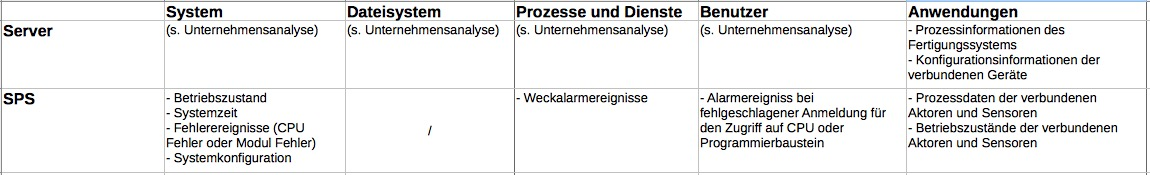
\includegraphics[width=125mm]{Zeichnungen/IndustriesystemInformationen.jpg}
\caption{Placeholder: Darstellung der verfügbaren Informationen der Systeme}
\label{fig:IndustrySystemInformation}
\end{figure}

\subsection{Netzwerkprotokolle}
%PROFINET
Zunächst wird das PROFINET Protokoll betrachtet. PROFINET basiert auf der Basis des Ethernet-Standards und abhängig von der verwendeten Konfiguration auf dem Internetprotokoll (IP) und einem Transportprotokoll (TCP oder UDP). Dementsprechend werden die im vorherigen Kapitel beschriebenen Kategorien für diese Protokolle verwendet und der Fokus bei der Kategoriezuweisung auf die Funktionalitäten gelegt. 
PROFINET unterscheidet verschiedene Konformitätsklassen. Für die Zuordnung werden jedoch zunächst alle potentiell verfügbaren, vorher beschriebenen Funktionen kategorisiert. Bei der späteren, vergleichenden Betrachtung werden die klassenspezifischen Funktionalitäten entsprechend markiert. \\

Zu der Header-Kategorie werden die Informationen aus den Headern hinzugezählt. Im Falle von PROFINET gehören zu diesen Informationen neben den Ebenen des TCP/IP-Stacks die Operationen Read und Write für Bedarfsdaten, Identifizierung und Verwaltung sowie Alarme für Geräte- und Kommunikationsfehler. \\

Bzgl. der Verhaltenskategorien werden außerhalb des Verhaltens der unterliegenden Standards die Kommunikation über die verschiedenen Kommunikationskanäle gewertet. Diese Zuweisung deckt einen Bereich ab, in dem potentiell Nachrichten mit für den Kommunikationskanal ungültigen Nachrichtenkopfeinträgen gesendet werden. Diese Information kann potentiell auf eine Manipulation der gesendeten Pakete hindeuten, wodurch die korrekte Verwendung relevant wird. \\

\todoQuestion{Industrieanalyse Kategorisierung: Gehören Informationen von Geräteprofildateien bzgl. verwendbarer Dienste auch zur Protokollkategorie Verhalten?}

%PROFIBUS
Für PROFIBUS gelten die oben gesetzten Vorbedingungen der verwendeten Standards nicht, da das Kommunikationssystem nicht auf diesen Standards beruht.\\

Eine PROFIBUS-Nachricht definiert im Nachrichtenkopf verschiedene Informationen. Dazu gehören u.a. die verschiedenen Nachrichtentypen (z.B. Quittung oder Token) sowie Funktionstypen, Telegrammformate und die Empfänger- und Senderadresse. Dementsprechend werden diese Informationen der Header-Kategorie zugeordnet.  

Zu der Verhaltenskategorie werden im Bezug auf PROFIBUS der Vorgang, das Einflechten und der Ablauf der azyklischen Kommunikation gewertet. Ein weiteres Verhaltensmerkmal ergibt sich aus dem Prozess des Hinzufügens und Entfernens von Teilnehmern aus dem Kommunikationsbus und weitere definierte Sequenzen (z.B. Slave-Initialisierung oder Alarmsequenzen). Eine interessante Frage stellt sich bzgl. der Änderung eines Betriebszustandes eines DPM1 Gerätes. Da der DPM1 Zustand propagiert bzw. ein entsprechender Ablauf durchgeführt wird, lässt sich diese Information aus einem Mitschnitt der Kommunikation auf dem Kommunikationsbus erhalten und dementsprechend zur Verhaltenskategorie zuordnen. Allerdings lässt sich der Zustand auch von dem entsprechenden Gerät abfragen. Da jedoch die Information zuerst durch den Kommunikationsablauf erhältlich wird und der Betriebszustand zur PROFIBUS Funktionalität gehört, werden die Betriebszustände bzw. Betriebszustandswechsel der Verhaltenskategorie zugeordnet.

Die folgende Tabelle zeigt die Kategorien im Bezug auf die in diesem Kapitel analysierten Protokolle:
\todoForm{Industriesanalyse: Tabelle aktualisieren und in Latex erstellen}

\begin{figure}[h]
\centering
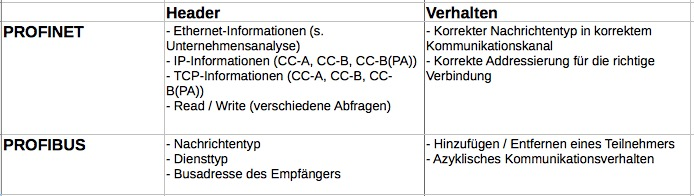
\includegraphics[width=125mm]{Zeichnungen/IndustrienetzwerkInformationen.jpg}
\caption{Placeholder: Darstellung der verfügbaren Informationen der Netzwerkprotokolle}
\label{fig:IndustryNetworkInformation}
\end{figure}